\chapter{Model Inference and Revision}\label{chap:modelInference}
\begin{mybox}
In the previous chapter, we introduced several approaches of refined reachability analysis, which are more suitable for practical use (more efficient and more conclusive).
Nevertheless, these approaches can never take effect no matter how powerful they are, if the original model does not reflect the reality.

To model a biological computational system, one may consider two possible aspects: a first-step model built by biologists (variables, some confirmed transitions, some \textit{a priori} properties etc.) and the observations from experiments (time-series data, steady states, oscillations, etc.).

This chapter is dedicated to the introduction of three different approaches of model inference/revision:

\begin{itemize}
    \item \textit{via} reachability properties and candidate regulations
    \item \textit{via} partial correlation (statistics)
    \item \textit{via} reachability properties and time-series data
\end{itemize}

There lies very little nuance between model inference and model revision: these two operations begin with some \textit{a priori} information and/or observations, aiming at constructing a new model/modifying an existed model.
As a result, they take the information apart from the existing transitions into account, using different tools to transform this information into possible transitions in the model (also can modify or deny existing transitions).

\end{mybox}

\section{Background}
Model inference/learning can be useful not only in biology \cite{ribeiro2015learning} but also in other domains with the need of abstraction, e.g. robotics \cite{nguyen2011model}, multi-agent systems \cite{foerster2016learning}.
In the community of bioinformatics, DREAM  challenge\footnote{\url{http://dreamchallenges.org/about-dream}} is a well-known organization calling for the participation of the whole world on the newest bio-medical problems (called challenges). 
Among these challenges, some of them are in the domain of inference and prediction:
DREAM2\footnote{\url{https://www.synapse.org/\#!Synapse:syn2825374/wiki/71143}},
DREAM4\footnote{\url{https://www.synapse.org/\#!Synapse:syn2825304/wiki/71129}},
DREAM8\footnote{\url{https://www.synapse.org/\#!Synapse:syn1720047/wiki/55342}},
DREAM11\footnote{\url{https://www.synapse.org/\#!Synapse:syn6131484/wiki/402026}}.

Like in biology, the modeling structures in robotics are usually complex and with big scale, which is difficult in control, prediction and simulation.
Constructing an abstracted (often approximated) model is a compromising way of dealing with the mechanical and computational complexity.
However, the abstracted models are theoretically non-equivalent to the original ones because they contain different amount of information.
Even though there always lies an non-equivalence, we wish that the abstracted models are in bisimulation with the original systems with respect to certain variables and keep the same important properties as original systems.

As is mentioned in Section \ref{sec:contribution} of Chapter \ref{chap:intro}, as far as we know, there has been no work combining model inference and model revision.
Some related works: Opgen-Rhein \textit{et als.} have \cite{opgen2007correlation} studied the undirectional inference \textit{via} correlation, Rodrigues \textit{et als.} \cite{rodrigues2011active} have studied the learning of action models and Bonneau \textit{et als.} \cite{bonneau2006inferelator} have studied the learning from continuous time-series data.

Figure \ref{fig:bigPicture} shows the methodology of this chapter.
There are two parallel pathways: 
\begin{itemize}
    \item One starts with biological \textit{a priori} knowledge.
    The knowledge comes from biological literature, certain empirical conclusion can be translated to temporal properties (especially reachability).
    \item The other one starts with partial observation.
    It is said partial because the real system is not completely observable, only a part of parameters can be taken as I/O. 
    Learning approaches will build a model consistent with partial observation but not necessarily consistent with the real system.
    Model checkers can verify the temporal properties and we can come up with some modifications to make the model consistent with \textit{a priori} knowledge.
\end{itemize}

\begin{figure}[ht]
    \centering
        \begin{tikzpicture}[line,>=stealth]
        \node [color=gray] (1) {Real system};
        \node [color=blue,right = of 1] (2) {Temporal properties};
        \node [below = 5cm of 1] (3) {Partial observation};
        \node [right = of 3] (4) {\textit{Learning methods}};
        \node [color=blue,right = of 2] (5) {Reachability};
        \node [below = 5cm of 5] (8) {Model};
        \draw [->] (4) -- (8);
        \node [color=blue,above = of 2] (6) {Biological \textit{a priori} knowledge};
        \draw [dashed,->] (1) -- (6);
        \draw [color=blue,->] (2) -- (5);
        \draw [dashed,->] (1) -- (3);
        \draw [->] (3) -- (4);
        \draw [color=blue, ->] (6) -- (2);
        \node [color=red, above = 2cm of 4] (7) {\textit{Model Checking}};
        \node [draw, circle, color = red, above = 2cm of 8] (9) {$+$};
        \draw [thick, color=red] (4) --(9);
        \draw [->] (5) --(7);
        \draw [thick, color=red] (7) --(9);
        \draw [thick, color=red] (9)--(8);
    \end{tikzpicture}
    \caption{Big picture of model inference}\label{fig:bigPicture}
\end{figure}

We developed two learning approaches following the Big Picture in Figure \ref{fig:bigPicture}.

\begin{itemize}
    \item CRAC (Completion \textit{via} Reachability And Correlations)
    
    CRAC is decomposed into two steps:
    \begin{enumerate}
        \item Infer candidate regulations from continuous time-series data
        \item Select transitions consistent with candidate regulations and add them into/delete them from an existing incomplete model (can be empty) to make it satisfy \textit{a priori} reachability information
    \end{enumerate}
    \item M2RIT (Model Revision \textit{via} Reachability and Interpretation Transitions)
    
    M2RIT is also run with two steps:
    \begin{enumerate}
        \item Learns a Normal Logic Program from \textit{discretized} time-series data by asynchronous version of LFIT (synchronous version in Section \ref{sec:lfitSyn})
        \item Modify the obtained NLP as little as possible to make it consistent with \textit{a priori} reachability information while keeping the consistency with the constraints of time-series data, i.e. the NLP has to reproduce the time-series data
    \end{enumerate}
\end{itemize}

It is worth noticing that step 2 of CRAC could be an individual model inference algorithm if the set of candidate regulations/transitions is given.
This step has the least complexity.
Because the most naive method, \textit{i.e.} brute force search is to verify every combination of the candidates if it satisfies the constraints. 
The models to be verified are of $O(2^n)$, where $n$ is the number of candidate transitions.

One may ask if we can run CRAC or M2RIT without being provided with time-series data, i.e. run directly step 2 of either method.
Deleting can be done without additional data, as the number of transitions already \textit{assuring} certain reachability is very limited, which is shown in Section \ref{sec:cutset} or \cite{PAK13-CAV}.

Nevertheless, adding transitions can be a more complex task.
Suppose we begin with no constraints on the model, to obtain a transition $A\to a_i$ with fixed $a_i$, there are at most $m-1$ possibilities for $A$ having one local state, $C_{m-1}^2$ possibilities for $A$ having 2 local states \ldots where $m$ is the number of model variables.
This factorial number of possibilities for \textbf{one} transition is not acceptable.

\section{Model Completion \textit{via} Candidate Regulations}\label{sec:modelInference}
We begin with the part which seems to have the smallest complexity.
Brute force search that we just presented is still meaningless in real application.
Roughly speaking, we prefer finding the transitions among the candidates which meet the unsatisfied constraints and keep already satisfied constraints unchanged.

\subsection{Problem Description}
Given an incomplete model, at first it does not satisfy wanted reachability properties.
With given set of candidade regulations, we can consider the transitions inferred by these candidates are more likely to be the good ones than the randomly generated ones.
Then we select the transitions which are prone to make certain unsatisfied reachability property satisfied and add them into the set of model transitions.

Briefly speaking, completion problem is:

incomplete model + candidate regulations + constraints $\to$ new model

The resulted model is expected to contain all the elements in the incomplete model and be consistent with all the \textit{a priori} information. 

\begin{definition}[Model completion in ABAN semantics]
    Given an incomplete ABAN $AB=(\Sigma, L, T)$ (where $T$ can be empty), a complete model is an ABAN $AB'=(\Sigma, L, T')$ which satisfies $T'\supseteq T$, $AB'$ consistent with the set of reachability constraints $C$ and the completion set $CS=T'\setminus T$ is consistent with the set of candidate regulations $R$, where
    \begin{itemize}
        \item $R=\{(body,head,sgn)\mid body\in \Sigma,\ head\in \Sigma,\ sgn\in \{-,+\}\}$ 
        \item $C=\{(\alpha,\omega,r)\mid\alpha \in L,\ \omega\in LS,\ r\in \{\mathbf{True,False}\}\}$
    \end{itemize}
\end{definition}

$R$ is the set of possible relations between variables, $body$ may inhibit ($sgn=-$) or promote ($sgn=+$) $head$.
$C$ is the set of reachability properties to be satisfied, $\omega$ is (un)reachable from $\alpha$.
The definition of consistency is straightforward, but its meaning changes for reachability constraints and candidate regulations.

\begin{definition}[Consistency]
\leavevmode
\makeatletter
\@nobreaktrue
\makeatother
\begin{itemize}
    \item An ABAN $AB$ is said consistent with the set of reachability constraints $C$ iff $\forall (\alpha,\omega,r)\in C$ s.t. $reach(\alpha,\omega)=r$
    \item A completion set $CS$ is said consistent with the set of candidate regulations $R$ if $\forall \acm{a_i}{b_{1-j}}{b_j}\in CS, \exists (body,head,sgn)\in R$ s.t. $body=a,\ head=b$ and $sgn=+$ if $i=j$, $sgn=-$ if $i\neq j$. 
\end{itemize}
    
\end{definition}

However, completion operation is not able to remove or modify existing trajectories towards the states to be reached as the transitions used in the trajectories are still present.
To obtain an ABAN meeting all the unreachable constraints in $C$, we have to apply cut sets.

Before our research began, Paulev\'e \textit{et al.} \cite{PAK13-CAV} had worked on cut-sets for reachability in large scale automata networks, which is the reverse operation of completion sets.
Cut set is used to eliminate certain transitions to make certain local states unreachable.

By combining these two operations, one can construct/revise a model according to \textit{a priori} information (candidate regulations) and constraints (reachability).

As stated in the previous chapter, verifying exact reachability is a hard task.
Here we use two metrics, over-approximation and under-approximation to replace and approach the notion of reachability (as shown in Figure \ref{fig:vennDiagram} on page \pageref{fig:vennDiagram}).

%In the context of SLCG, completion is defined as follows: given a state sequence $S$ of observation and a set of possible regulations $H$ (in the form of ABAN) to be verified, find the minimum subset of $H$ such that $S$ is realizable from initial state.

\subsection{Completion by Over-Approximation}
Over-approximation is the reasoning of pseudo-reachability in Definition \ref{defPseudoReach} on page \pageref{defPseudoReach}. 
It associates local states and transitions with the initial state according to the causalities: if there exists a reverse pathway from the target local state to the initial state, this target state can be reachable.
Over-approximationdoes not take into consideration the order of transitions to be fired, which is the cause of inconclusiveness (literally it over-approximates the reachability).
Thus over-approximation is a necessary condition of the reachability.

Figure \ref{CompOv} gives a first impression of the idea.
The visualization of the set of candidate regulations $R=\{(a,b,+),(c,a,-)\}$ is on the left.
On the right, the initial ABAN has only three Boolean variables $\Sigma=\{a,b,c\}$ and initial state $\langle a_0,b_0,c_0\rangle$, with transitions $T=\{\acm{a_1}{b_0}{b_1}\}$.
$b_1$ is not reachable because of the unreachability of $a_1$.
As $(c,a,-)\in R$, consistent transition \ac{c_0}{a_0}{a_1} is added then $a_1$ becomes reachable which makes $b_1$ also reachable.
$T'=\{\acm{a_1}{b_0}{b_1},\acm{c_0}{a_0}{a_1}\}$, $CS=\{\acm{c_0}{a_0}{a_1}\}$.

\begin{figure}[ht]
\centering
\begin{minipage}{0.5\linewidth}
\centering
\begin{tikzpicture}
\coordinate (P1) at (0,0);
\node at (P1) {{\Large c}};
\coordinate (P2) at (2,0);
\node at (P2) {{\Large a}};
\coordinate (P3) at (4,0);
\node at (P3) {{\Large b}};
\coordinate (P4) at ($(P2)+(150:0.6)$);
\draw (P1) circle(0.4) ;
\draw (P2) circle(0.4);
\draw (P3) circle(0.4);
\draw [line width=1pt](30:0.5) .. controls  (1,0.7) .. (P4);
\draw [->, line width=1pt]($(P2)+(30:0.5)$) .. controls  (3,0.7) .. ($(P3)+(150:0.55)$);
\draw [line width=1pt]($(P4)+(45:0.15)$) -- ($(P4)-(45:0.15)$);
\end{tikzpicture}
\end{minipage}
\hfill
\begin{minipage}{0.5\linewidth}
\centering
\begin{tikzpicture}
\TSort{(0,0)}{c}{2}{l}
\TSort{(2,0)}{a}{2}{r}
\TSort{(4,0)}{b}{2}{r}
\THit{a_1}{}{b_0}{.west}{b_1}
\THit{c_0}{dashed,thick,color=red}{a_0}{.west}{a_1}


\path[bounce,bend left]
\TBounce{b_0}{}{b_1}{.west}
\TBounce{a_0}{thick,color=red}{a_1}{.west}
;
\TState{a_0,b_0,c_0}
\end{tikzpicture}
\end{minipage}

\caption[Completion by over-approximation]{Completion by over-approximation. Dashed arrows represent added action.}\label{CompOv}
\end{figure}
Algorithm \ref{algComOver} in Appendix shows the detailed algorithm of the completion by over-approximation.

\subsection{Completion by Under-Approximation}
Over-approximation is only a necessary condition of reachability.
If one wants the guarantee of the reachability even at the price of redundant transitions, he may consider the completion by under-approximation.

Under-approximation is another reasoning of SLCG. 
It associates the local states and the transitions with the initial state and \textit{all the states which may appear}.
This association covers all the orders of occurrence (proof is given in Theorem \ref{th:underapprox} of Appendix).
Similar to over-approximation, in the SLCG of under-approximation, if there is a pathway between target local state and the initial state, this target state \textit{should} be reachable.

However, all the orders of occurrence do not necessarily appear during the simulation, which suggest that this approach ``under-approximates'' the reachability.

Additionally, the computation of under-approximation is more complicated than that of over-approximation, as the set of associated local states grows during the computation.
Former added local states need to be regarded as new ``target states''.
This process is called \textit{update}. 
Update does not stop until the set of associated local states becomes stable.


\begin{definition}[Under-approximate SLCG]
Given ABAN $AB = (\Sigma,L,T)$, a global initial state $\alpha$ and a target local state $\omega$, under-approximate SLCG $l= (V_{\mathrm{state}},V_{\mathrm{solution}},E)$ is the smallest recursive structure with $E \subseteq (V_{\mathrm{state}}\times V_{\mathrm{solution}})\cap (V_{\mathrm{solution}}\times V_{\mathrm{state}})$ which satisfies:
\begin{eqnarray*}
    \omega&\in& V_{\mathrm{state}} \\
    a_i\in V_{\mathrm{state}} &\Leftrightarrow& \{ (a_i, sol_{a_i}| head(sol_{a_i})=a_i)\}\subseteq E \\
    sol_{a_i}\in V_{\mathrm{solution}}&\Leftrightarrow& \{ (sol_{a_i},\mathbf{V}(sol_{a_i}))| \mathbf{V}(sol_{a_i})=\varnothing \text{ \rm if } a_i\in \alpha\land a_{1-i}\not\in V_{\mathrm{state}},\\
    &&\text{ \rm else }\mathbf{V}(sol_{a_i})\in body(sol_{a_i}) \}\subseteq E
\end{eqnarray*}
where $V_{\mathrm{state}}\subseteq LS$ is a set of local states, $V_{\mathrm{solution}}\subseteq T$ is the a of solutions and $\mathbf{V}(sol_{a_i})$ is the set of required local states of $sol_{a_i}$. 
\end{definition}

If we compare the definition of under-approximation with Definition \ref{defSLCG} of over-approximation on page \pageref{defSLCG}, the difference lies in the condition of $\mathbf{V}(sol_{a_i})$. 
The reasoning of over-approximation stops when certain automaton $a$ reaches the initial state. 
However, to guarantee all the possible orders, we exige $a_i$ and $a_{1-i}$ are reachable from each other if they are both present in the under-approximate SLCG.
The corresponding formula is $\mathbf{V}(sol_{a_i})=\varnothing \text{ \rm if } a_i\in \alpha\land a_{1-i}\not\in V_{\mathrm{state}}$.

The visualization of under-approximate SLCGs has a slight difference with the one of over-approximate SLCGs.
$a_0\Rsh a_1$ means $a_1$ is to be reached \textit{via} $a_0$.
This notation seems redundant but it is useful when we need to continue the reasoning even if we reach the initial state until the SLCG is saturated.
Local states in the initial state may have other successors besides $\bigcirc$.
For example in Figure \ref{Under2}, $d_0$ is in the initial state, but the reasoning continues because $d_1$ appears in another branch.

\begin{example}
Given ABAN $AB=(\Sigma, L, T)$ in Figure \ref{ExUnder} with $\Sigma= \{a,b,c,d\}$, $T=\{\acm{b_1,c_1}{a_0}{a_1}, \acm{b_1}{d_0}{d_1}, \acm{d_0}{b_0}{b_1}\}$, the initial state $\langle a_0,b_0,c_0,d_0\rangle$.
With candidate regulations $R=\{(d,c,-),(c,d,-)\}$, Figure \ref{Under1}, Figure \ref{Under2} and Figure \ref{Under3} show the procedures of completion by under-approximation: after two additions of actions and one update, the SLCG becomes stable and $a_1$ becomes reachable.
$T'=\{\acm{b_1,c_1}{a_0}{a_1}, \acm{b_1}{d_0}{d_1}, \acm{d_0}{b_0}{b_1},\acm{d_1}{c_0}{c_1}, \acm{c_1}{d_1}{d_0}\}$, $CS=\{\acm{d_1}{c_0}{c_1}, \acm{c_1}{d_1}{d_0}\}$.

\begin{figure}[ht]
\centering
%\begin{tikzpicture}
%\TSort{(3,0)}{a}{3}{l}
%\TSort{(0,0)}{b}{2}{l}
%\TSort{(6,0)}{c}{2}{r}
%\TSort{(2,-2)}{d}{2}{b}
%\THit{b_1}{}{a_0}{.north west}{a_1}
%\THit{c_1}{}{a_1}{.east}{a_2}
%\THit{d_0}{distance=90,out=240,in=210}{b_0}{.west}{b_1}
%\THit{b_1}{}{d_0}{.north}{d_1}
%\THit{d_0}{distance=90,out=-75,in=-45,dashed,thick,color=red}{c_0}{.east}{c_1}
%\THit{c_1}{dashed,thick,color=red}{d_1}{.north}{d_0}
%
%
%\path[bounce,bend right]	
%\TBounce{a_1}{}{a_2}{.east}
%\TBounce{d_1}{thick,color=red}{d_0}{.north east}
%\TBounce{c_0}{thick,color=red}{c_1}{.east}
%;
%\path[bounce,bend left]
%\TBounce{a_0}{}{a_1}{.west}
%\TBounce{b_0}{}{b_1}{.west}
%\TBounce{d_0}{}{d_1}{.north west}
%;
%\TState{a_0,b_0,c_0,d_0}
%\end{tikzpicture}
\begin{tikzpicture}[apdotsimple/.style={apdot}]
\scriptsize
\TSort{(0,0)}{a}{2}{l}
\TSort{(2,0)}{b}{2}{l}
\TSort{(4,0)}{c}{2}{l}
\TSort{(6,0)}{d}{2}{l}

% with delays
\path[local transitions]

	(a_0) edge node[auto] {\{$b_1, c_1$\}} (a_1)
	
	(b_0) edge node[auto] {$\{d_0\}$} (b_1)
	(d_0) edge node[auto] {$\{b_1\}$} (d_1)
	(d_1) edge[dashed,color=red] node[auto] {$\{c_1\}$} (d_0)
	%(c_1) edge node[auto] {$\{b_0\}$, $2$} (c_0)
	(c_0) edge[dashed,color=red] node[auto] {$\{d_1\}$} (c_1)
;

\TState{a_0, b_0, c_0, d_0}


\end{tikzpicture}

\caption[Completion by under-approximation]{Example of completion by under-approximation. Dashed arrows represent added transitions.}\label{ExUnder}
\end{figure}

Figure \ref{Under1} shows the under-approximate SLCG of the reachability $a_1$.
\fbox{$c_1$} is unreachable then the joint state $\langle b_1, c_1\rangle$ is not reachable, $a_1$ is not reachable.

\begin{figure}[ht]
\centering
\begin{tikzpicture}
\node (O1) at (0,0) {$a_0\Rsh^*a_2$};
\node[draw] (Pm1) at (-1.75,0) {$a_2$};
\draw[->] (Pm1)-- (O1);
\node (S1) at ($(O1)+(1.5,0)$){};
\draw[->] (O1) -- (S1);
\draw (S1) circle (3pt);
\node[draw] (P1) at ($(S1)+(1,1)$){$b_1$};
\node[draw] (P2) at ($(S1)+(1,-1)$){$c_1$};
\draw[->] (S1)--(P1);
\draw[->] (S1)--(P2);
\node (O2) at ($(P1)+(1.75,0)$) {$b_0\Rsh^*b_1$};
\node (O3) at ($(P2)+(1.75,0)$) {$\perp$};
\draw[->] (P1)--(O2);
\draw[->] (P2)--(O3);
\node (S2) at ($(O2)+(1.5,0)$){};
\draw (S2) circle (3pt);
\draw[->] (O2) -- (S2);
\node[draw] (P3) at ($(S2)+(1,0)$){$d_0$};
\draw[->] (S2) -- (P3);
\node (O5) at ($(P3)+(1.75,0)$) {$d_0\Rsh^*d_0$};
\draw[->] (P3)--(O5);
\node (S5) at ($(O5)+(1.5,0)$){};
\draw (S5) circle (3pt);
\draw[->] (O5) -- (S5);
\end{tikzpicture}
\caption[Operations on SLCG(1)]{Step 1, under-approximation S of Figure \ref{ExUnder} studying the reachability of $a_1$ (small circles stand for solutions and squares stand for required local states). }\label{Under1}
\end{figure}

In Figure \ref{Under2}, according to candidate regulation ${(d,c,-)}\in R$, transition \ac{d_1}{c_0}{c_1} is added.
Thanks to the existence of \ac{b_1}{d_0}{d_1}, $d_1$ has successor $b_1$.
However, the reachability of under-approximation requires all the possible occurrences are realizable, i.e. we need a transition with body $d_0$ for $d_0$ and $d_1$ can be reached from each other, because both $d_0$ and $d_1$ are present in the SLCG.


\begin{figure}[ht]
\centering
\begin{tikzpicture}
\node (O1) at (0,0) {$a_0\Rsh^*a_1$};
\node[draw] (Pm1) at (-1.75,0) {$a_1$};
\draw[->] (Pm1)-- (O1);
\node (S1) at ($(O1)+(1.5,0)$){};
\draw[->] (O1) -- (S1);
\draw (S1) circle (3pt);
\node[draw] (P1) at ($(S1)+(1,1)$){$b_1$};
\node[draw] (P2) at ($(S1)+(1,-1)$){$c_1$};
\draw[->] (S1)--(P1);
\draw[->] (S1)--(P2);
\node (O2) at ($(P1)+(1.75,0)$) {$b_0\Rsh^*b_1$};
\node (O3) at ($(P2)+(1.75,0)$) {$c_0\Rsh^*c_1$};
\draw[->] (P1)--(O2);
\draw[->] (P2)--(O3);
\node (S2) at ($(O2)+(1.5,0)$){};
\draw (S2) circle (3pt);
\draw[->] (O2) -- (S2);
\node (S3) at ($(O3)+(1.5,0)$){};
\draw[fill=black] (S3) circle (3pt);
\draw[->] (O3) -- (S3);
\node[draw] (P3) at ($(S2)+(1,0)$){$d_0$};
\draw[->] (S2) -- (P3);
\node[draw] (P4) at ($(S3)+(1,0)$){$d_1$};
\draw[->] (S3) -- (P4);
\node (O4) at ($(P3)+(30:1.75)$) {$d_0\Rsh^*d_0$};
\node (O5) at ($(P3)+(1.75,0)$) {$d_1\Rsh^*d_0$};
\draw[->] (P3)--(O4);
\draw[->] (P3)--(O5);
\node (O6) at ($(P4)+(-30:1.75)$) {$d_1\Rsh^*d_1$};
\node (O7) at ($(P4)+(1.75,0)$) {$d_0\Rsh^*d_1$};
\draw[->] (P4)--(O6);
\draw[->] (P4)--(O7);
\node (S4) at ($(O4)+(1.5,0)$){};
\draw (S4) circle (3pt);
\draw[->] (O4) -- (S4);
\node (S5) at ($(O5)+(1.5,0)$){$\perp$};
\draw[->] (O5) -- (S5);
\node (S6) at ($(O6)+(1.5,0)$){};
\draw[fill=black] (S6) circle (3pt);
\draw[->] (O6) -- (S6);
\node (S7) at ($(O7)+(1.5,0)$){};
\draw[fill=black] (S7) circle (3pt);
\draw[->] (O7) -- (S7);
\draw[->] ($(S7)+(0,3pt)$) -- (P1);
\end{tikzpicture}
\caption[Operations on SLCG(2)]{Step 2 of completion by under-approximation (filled small circles stand for new possible solutions after completion).}\label{Under2}
\end{figure}

In Figure \ref{Under3}, the completed under-approximate SLCG shows $a_1$ is now reachable after adding $\acm{c_1}{d_1}{d_0}$ according to ${(c,d,-)}\in R$ as there is no more $\perp$ in the SLCG.

\begin{figure}[ht]
\centering
\begin{tikzpicture}[>=stealth]
\node (O1) at (0,0) {$a_0\Rsh^*a_1$};
\node[draw] (Pm1) at (-1.75,0) {$a_1$};
\draw[->] (Pm1)-- (O1);
\node (S1) at ($(O1)+(1.5,0)$){};
\draw[->] (O1) -- (S1);
\draw (S1) circle (3pt);
\node[draw] (P1) at ($(S1)+(1,1)$){$b_1$};
\node[draw] (P2) at ($(S1)+(1,-1)$){$c_1$};
\draw[->] (S1)--(P1);
\draw[->] (S1)--(P2);
\node (O2) at ($(P1)+(1.75,0)$) {$b_0\Rsh^*b_1$};
\node (O3) at ($(P2)+(1.75,0)$) {$c_0\Rsh^*c_1$};
\draw[->] (P1)--(O2);
\draw[->] (P2)--(O3);
\node (S2) at ($(O2)+(1.5,0)$){};
\draw (S2) circle (3pt);
\draw[->] (O2) -- (S2);
\node (S3) at ($(O3)+(1.5,0)$){};
\draw (S3) circle (3pt);
\draw[->] (O3) -- (S3);
\node[draw] (P3) at ($(S2)+(1,0)$){$d_0$};
\draw[->] (S2) -- (P3);
\node[draw] (P4) at ($(S3)+(1,0)$){$d_1$};
\draw[->] (S3) -- (P4);
\node (O4) at ($(P3)+(30:1.75)$) {$d_0\Rsh^*d_0$};
\node (O5) at ($(P3)+(1.75,0)$) {$d_1\Rsh^*d_0$};
\draw[->] (P3)--(O4);
\draw[->] (P3)--(O5);
\node (O6) at ($(P4)+(-30:1.75)$) {$d_1\Rsh^*d_1$};
\node (O7) at ($(P4)+(1.75,0)$) {$d_0\Rsh^*d_1$};
\draw[->] (P4)--(O6);
\draw[->] (P4)--(O7);
\node (S4) at ($(O4)+(1.5,0)$){};
\draw (S4) circle (3pt);
\draw[->] (O4) -- (S4);
\node (S5) at ($(O5)+(1.5,0)$){};
\draw[fill=black] (S5) circle (3pt);
\draw[->] (O5) -- (S5);
\node (S6) at ($(O6)+(1.5,0)$){};
\draw (S6) circle (3pt);
\draw[->] (O6) -- (S6);
\node (S7) at ($(O7)+(1.5,0)$){};
\draw (S7) circle (3pt);
\draw[->] (O7) -- (S7);
\draw[->] ($(S5)-(0,3pt)$) -- (P2);
\draw[->] ($(S7)+(0,3pt)$) -- (P1);
\end{tikzpicture}
\caption[Operations on SLCG(3)]{Step 3 of completion by under-approximation (filled small circles stand for new possible solutions after completion).}\label{Under3}
\end{figure}
\end{example}

To sum up the whole process, we begin with a incomplete model and a set of candidate regulations.


Algorithm \ref{algComUnder} in Appendix shows the detailed procedures of completion by under-approximation.

\begin{remark}
Neither completion by under-approximation nor completion by over-approximation can output complex transitions (transitions with multiple variables in the head).
If one wants to assess if certain complex transition can be added to the incomplete model, he can replace regulations in the input with transitions, skip the step of checking the consistency, then use directly the transition to complete the incomplete model.
\end{remark}

\section{Model Inference via Statistics}
As we already have the completion methods, to make CRAC applicable, we need to obtain candidate regulations $R$.
Here we introduce a method to generate candidate regulations to be verified from time series data.

In the previous contents, only the systems consisting of transitions with delay of 1 time unit are discussed (BN, ABAN, etc.), i.e. the influence done by variables will take place at the next time point (immediately).
However, in biological context, some reactions have a long duration, and some even need a whole observation period to take place.
For this reason, we require approaches to reveal transitions of different delays: for an observation of period $T$, possible delays lie in $[1,T-1]$.

\subsection{Preliminaries}
In Definition \ref{def:RN} on page \pageref{def:RN}, the definition of regulatory network (RN) is originally related to a set of approximated ordinary differential equations (ODEs) \cite{khalis2009smbionet} (continuous modeling):
%$$\dv{x_v}{t}=k_v+\sum_{u\in v.pred}{x_uk_{uv}s^{\alpha_{uv}}(x_u,\theta_{uv})}-\lambda_v x_v$$
\begin{equation}\label{eq:differentialEquation}
    \dv{x_v}{t}=k_v-\lambda_v x_v +\sum_{u\in v.pred}{x_uk_{uv}}
\end{equation}

where $x_v$ is the concentration of variable $v$, $k_v, \lambda_v\in \mathbb{R}$ are self-regulation kinetic parameters and $k_{uv}\in \mathbb{R}$ are kinetic parameters of external regulations.

%\begin{itemize}
%    \item $k_v\in \mathbb{R^{*}}$ and $k_{uv}\in \mathbb{R^{+*}}$ are kinetic parameters
%    \item the function $s^{\alpha_{uv}}$ gives the effect of a regulator $u$ and its target $v$.
%    This function is usually a sigmoid depending on the sign $\alpha_{uv}$ and on the quantitative threshold $\theta_{uv}\in \mathbb{R}^{+*}$ the interaction.
%\end{itemize}

Here, considering the following reasons, we make several modifications to the ODE.
\begin{enumerate}
    \item The change rate done by external regulations is not always proportional to the concentration of corresponding external variables. 
    Consider an elementary biochemical reaction $m\mathrm{A}+n\mathrm{B}\rightarrow \mathrm  {C}$, according to the rate law, the synthesis rate of C is $r_{\mathrm{C}}=k[{\mathrm{A}}]^{m}[{\mathrm{B}}]^{n}$ where $k$ is a fixed positive real number and $m,n$ are the parameters characterizing reaction order.
    \item In the community of model inference, self-regulations are often considered difficult to be detected because nearly every transition could be explained as the result of a self-regulation.
    For example, in the problem description of DREAM8\footnote{\url{https://www.synapse.org/\#!Synapse:syn1720047/wiki/55342}}, self-regulations are \textit{a priori} ignored.  
    \item According to the differential equation, the influence takes effect immediately without delay.
    However, considering the discretization on time, we have to replace the differential mark $\mathrm{d}$ in \ref{eq:differentialEquation} into difference mark $\Delta$ and set a delay $\delta$ which takes only natural numbers to simulate state change.
\end{enumerate}

To integrate these hypotheses, the equations are modified to:

%$$\dv{x_v}{t}=\sum_{u\in v.pred}{k_{uv}s^{\alpha_{uv}}(x_u,\theta_{uv})}$$
%$$\dv{x_v(t)}{t}=\sum_{u\in v.pred}{x_u(t)k_{uv}}$$
\begin{equation}\label{eq:differenceEquation}
    \frac{\Delta{x_v(t)}}{\Delta t}=\sum_{u\in v.pred}{x_u^{n}(t-\delta)k_{uv}}
\end{equation}


where $\delta\in \mathbb{N}^{*}$ is the delay of the regulation, $n\in \mathbb{R}^{+}$ is the order of regulation (corresponding to the reaction order).
Also, self-regulations are not taken into account, i.e. $k_v$ and $\lambda_v$ are set to 0.

The definition of RN (Definition \ref{def:RN}) requires every regulation take effect immediately.
To cooperate with the new equations, it is adapted to the version with delay.

\begin{definition}[Regulatory network with delay]
A regulatory network with delay is a labeled directed graph $G=(V,E)$ where 
\begin{itemize}
    \item each vertex $v$ of $V$, called variable, is provided with a boundary $b_v\in \mathbb{N}$ less or equal to the out-degree of v in G.
    \item each arc $u\in v$ of $E$ is labelled with a triplet ($t_{uv}, \alpha_{uv}, \delta$) where $t_{uv}$ is an integer between 1 and $b_v$, called qualitative threshold, where $\alpha_{uv}\in \{+,-\}$ is the sign of the regulation and $\delta\in \mathbb{N^+}$ is the delay of the regulation.
\end{itemize}
\end{definition}

With the new formalization, we can now address the inference problem.

\subsection{Partial Correlation}

In huge biological networks, it is not possible to compute candidate regulations by hand nor to traverse all the possible addable transitions, as stated formerly, the verification of $O(3^{|Global States|})$ states is a huge task: if the influenced variable is fixed, every other variable has 3 possible influence, promotion, inhibition and no regulation.
 
To deal with the high complexity of the verification of $O(3^{|Global States|})$ states, \textit{a priori} knowledge is needed. 
Some unsatisfied states can be eliminated without global verification.  
In order to take all the information into account, statistical approaches come into sight.
We use correlation coefficients to try to match the evolution of variables with Equation \ref{eq:differenceEquation} on page \pageref{eq:differenceEquation}.
Correlation coefficients characterizes how linear or monotonous the relations between variables are all along the sampling period.
The possible values of all the mentioned correlation coefficients lie in the interval $[-1,1]$.
The closer to $1$ the absolute value of the coefficient is, the more correlated the variables are.
Particularly, $1$ suggests total positive correlation and $-1$ suggests total negative correlation. 

In Equation \ref{eq:differenceEquation}, for different $n$,
\begin{enumerate}
    \item $n=1$, the change rate of certain variable is the linear sum of other variables.
    The \textit{linear} correlation between the change rate of one variable and the value of other variables is detectable via an approach using Pearson correlation coefficients (PCC).
    \item $n\neq 1$, the correlations between variables are no longer linear but still monotonous.
    Analogously the \textit{monotonous} correlation is detectable by Spearman correlation coefficients (SCC), which is the application of Pearson correlation coefficients on the rank of variables.
\end{enumerate}

One additional profit of statistical approaches is that original time series data are discretized before being used, which cause a loss of information.
This loss could lead to an imprecise model.
However, some statistical approaches could use directly the continuous time series data as input which avoid this drawback.

\begin{definition}[Pearson correlation coefficient]
    Pearson correlation coefficient ($r$) is the covariance of the two variables divided by the product of their standard deviations.
    When applied to a sample (time series data), the formula is converted to:
    $${\displaystyle r_{x,y}={\frac {\operatorname {cov} (x,y)}{\sigma _{x}\sigma _{y}}}={\frac {\sum _{i=1}^{N}(x_{i}-{\bar {x}})(y_{i}-{\bar {y}})}{{\sqrt {\sum _{i=1}^{N}(x_{i}-{\bar {x}})^{2}}}{\sqrt {\sum _{i=1}^{N}(y_{i}-{\bar {y}})^{2}}}}}}$$
    Where $x,y$ are variables, $\operatorname {cov} (x,y)$ is the covariance of $x$ and $y$, $\sigma _{x}$ is the standard deviation of $x$, $N$ is the sample size and $x_i,y_i$ are the $i$-th sample points of $x,y$.
\end{definition}

The definition of Spearman correlation coefficient is related to that of Pearson correlation coefficient.

\begin{definition}[Spearman correlation coefficient]
    Spearman correlation coefficient ($rs$) is the Pearson correlation coefficient between the ranked variables.
    $${\displaystyle rs_{x,y}=r_{\operatorname {rg} _{x},\operatorname {rg} _{y}}={\frac {\operatorname {cov} (\operatorname {rg} _{x},\operatorname {rg} _{y})}{\sigma _{\operatorname {rg} _{x}}\sigma _{\operatorname {rg} _{y}}}}}$$
    Where $rg_x$ is the rank variable of $x$.
\end{definition}

\begin{example}
Variable $x=\{3,10,1,7,6\}$, the rank variable of $x$ is $rg_x=\{4,1,5,2,3\}$.
\end{example}


If two variables are highly correlated and form an independent system, their correlation can be perfectly detected by PCC or SCC.
However, variables are usually simultaneously influenced by more than one variables, which is the biological reality.
For example, for three variables $a,b,c$, if $a$ is activated by $b$ and inhibited by $c$, the PCC or SCC of $r_{\ddv{a}{t},b}$ is biased by $c$. 
To get rid of certain variables, one can apply partial Pearson correlation coefficients \cite{baba2004partial} or partial Spearman correlation coefficients \cite{borror2001practical}.

Partial correlation coefficients are denoted $pr$.

\begin{definition}[Partial Pearson correlation coefficient (PPCC)]\label{def:PPCC}
    $pr_{xy\cdot \mathbf {z}}$ is the partial Pearson correlation coefficient of $x$ and $y$ ignoring the influence by $\mathbf {z}$.
    $$pr _{xy\cdot \mathbf {z} }={\frac {pr _{xy\cdot \mathbf {z} \setminus \{z_{0}\}}-pr _{xz_{0}\cdot \mathbf {z} \setminus \{z_{0}\}}pr _{z_{0}y\cdot \mathbf {z} \setminus \{z_{0}\}}}{{\sqrt {1-pr _{xz_{0}\cdot \mathbf {z} \setminus \{z_{0}\}}^{2}}}{\sqrt {1-pr _{z_{0}y\cdot \mathbf {z} \setminus \{z_{0}\}}^{2}}}}}$$
    Where $x,y$ are variables, $\mathbf {z}$ is a set of variables, $z_0$ is an arbitrary element in $z$. 
    Particularly, if $\mathbf {z}$ has only one element $z_0$, the formula becomes
    $$pr_{x,y\cdot \{z_0\}}={\frac {r _{x,y}-r _{x,z_0}r _{z_0,y}}{{\sqrt {1-r _{x,z_0}^{2}}}{\sqrt {1-r _{z_0,y}^{2}}}}}$$

\end{definition}

The partial Spearman correlation coefficient is defined likewise.
\begin{definition}[Partial Spearman correlation coefficient (PSCC)]\label{def:PSCC}
Partial Spearman correlation coefficient is denoted $prs$
    $$prs_{x,y\cdot \mathbf {z}}=pr_{rg_x,rg_y\cdot rg_\mathbf {z}}$$%={\frac {r _{rg_x,rg_y}-r _{rg_x,rg_z}r _{rg_z,rg_y}}{{\sqrt {1-r _{rg_x,rg_z}^{2}}}{\sqrt {1-r _{rg_z,rg_y}^{2}}}}}$$
\end{definition}

The possible value of all the mentioned correlation coefficients are in the interval $[-1,1]$.
The closer to $1$ the absolute value of the coefficient is, the more correlated the variables are.
Particularly, $1$ suggests total positive linear/monotonous correlation and $-1$ suggests total negative linear/monotonous correlation. 
e.g. if we find the PSCC of $\ddv{a}{t}$ and $b$ is $-0.9$ (high enough), we can add $b\xrightarrow{-}a$ to the set of candidate regulations.

\subsubsection{Overall Process}

With the former definitions, we propose a method applying partial correlation to detect the relevance of each pair of variables.

\begin{figure}[ht]
\begin{tikzpicture}[node distance = 1.5cm, auto]
    % Place nodes
    \node [block] (originalData) {Time-series data};
    \node [block, right = of originalData] (dataDiscretization) {Data discretization};
     \node [block, right = of dataDiscretization] (varReconstruction) {Variable reconstruction};
    \node [block, below = of originalData] (ranking) {Sorting};
    \node [block, right = of ranking] (changeRate) {Change rate};
    \node [block, below = of ranking] (dataReg) {Data regrouping \& Spearman coefficient};
     \node [block, right = of dataReg] (partialCoeff) {Partial coefficient};
     \node [block, right = of partialCoeff] (regulations) {Regulations $x\xrightarrow{+/-}y$};
     \node [block, below = of varReconstruction] (actions) {Transitions \ac{x_i}{y_j}{y_k}};
     \coordinate [left = of ranking,node distance=0.5cm](abstract);
    % Draw edges
    \path [line] (originalData) -- (dataDiscretization);
    \path [line] (originalData) -- (ranking);
    \path [line] (originalData) -- (changeRate);
    \path [line] (changeRate) -- (ranking);
    \path [line,dashed] (dataDiscretization) -- (varReconstruction);
    \path [line] (varReconstruction) -- (ranking);
    \path [line] (ranking) -- (dataReg);
    \path [line] (dataReg) -- (partialCoeff);
    \path [line] (partialCoeff) -- (regulations);
    \path [line,dashed] (regulations) -- (actions);
    \path [line,dashed] (originalData) -|  (abstract)node[rotate=90,below=2pt]{Pearson Coefficient} |-(dataReg);
\end{tikzpicture}
\caption[Workflow of model inference via partial correlation]{Workflow of the whole procedure of candidate regulations generation (dashed arrows stand for optional processes)}\label{plan}
\end{figure}

Figure \ref{plan} shows the procedure of regulation generation: before discretizing original data, Pearson or Spearman correlation coefficients \cite{samaga2009logic,hauke2011comparison} are computed for identifying the relevance between original data and change rates of variables (in linear or monotonic way respectively). If cooperation between variables exists, former coefficients need replacing by partial ones \cite{de2004discovery} for more precise result.
Resulting coefficients above the threshold (One can set a threshold of correlation, e.g. 0.7) suggest there probably exist regulations between variables.

Furthermore, to complete Biological Regulatory Networks in the form of ABAN, more accurate regulations are inferred through variable reconstruction, which splits a variable into several new variable according to its qualitative levels.
For example, variable $a$ has two discrete levels $a_0$ $a_1$, then the correlation coefficients as well as the partial coefficients are computed in the domain of $a_0$ and of $a_1$ separately.
As a result, the correlation between $a_0$ and other variables and that of $a_1$ are computed, with which candidate transitions are deduced.

As all the subroutines depicted in Figure \ref{plan} are defined, starting from original data, regulations in form of Ren\'e Thomas' model \cite{thomas1978} or ABAN are resulted step by step. In the next section, the data processing in Figure \ref{plan} will be introduced with examples.

\subsubsection*{Data Regrouping}
To gain a better understanding of correlations between observation data and change rate, certain observed data of one variable are replaced by corresponding change rate. By calculating the correlation coefficients of such matrix, regulation on this variable is characterized.

\begin{definition}[Regrouping]
    Let $A$ be a $n\times T$ matrix, representing time-series data, where $n$ is the number of variables and $T$ is the period of the time-series data.
    $A_{ij}$ is the $i$-th variable at time $j$. 
    Let $\delta$ be the delay we want to explore, there are in total $n$ matrices of size $n\times (T-\delta)$ after regrouping.
    The $k$-th matrix $A^{'k}$ is defined:
    
    \begin{equation}
    \nonumber
    A^{'k}_{ij}=
    \begin{cases}
        \dfrac{A_{i,j+\delta}-A_{ij}}{\delta} & {\rm if\ } i=k\\
         A_{ij} & {\rm if\ } i\neq k
    \end{cases}
\end{equation}
\end{definition}

We regroup the change rate of one variable and the values of the other variables in order to infer the correlations between them.

\begin{example}
Let us take the time-series data of 4 variables $a,b,c,d$ as an example.
Matrix $A$ below records the state of the system of discrete time point $t=0,1,2,3$, $A'^1$ is the first regrouped matrix ($k=1$) as the time-series of $a$ is placed on the first row.
$A'^1$ is used to compute the correlation between the change rate of $a$ and other variables of delay $\delta=1$.

\begin{equation}\label{eq:changeRate}
    a'(t)=\dfrac{\Delta a(t)}{\Delta t}=\dfrac{a(t+1)-a(t)}{(t+1)-t}=a(t+1)-a(t)
\end{equation}

$$A=\kbordermatrix{\mbox{\footnotesize$t$}&0&1&2&3\\
a&a(0)&a(1)&a(2)&a(3)\\
b&b(0)&b(1)&b(2)&b(3)\\
c&c(0)&c(1)&c(2)&c(3)\\
d&d(0)&d(1)&d(2)&d(3)
}
\to A'^1=\kbordermatrix{\mbox{\footnotesize$t$}&0&1&2\\
a'&a'(0)&a'(1)&a'(2)\\
b&b(0)&b(1)&b(2)\\
c&c(0)&c(1)&c(2)\\
d&d(0)&d(1)&d(2)
}$$

In this way, regulations of $b,c,d$ on $a$ are then evaluated by PPCC or PSCC (see Def \ref{def:PPCC} and \ref{def:PSCC}).
\end{example}

With the matrices $A'^k$, we can compute the matrix containing the correlation information of all the variable pairs.

\begin{definition}[Correlation matrix]\label{def:corrMatrix}
    Let $A'^k$ be the regrouped matrices of time-series data matrix $A$ with $k\in [1,n]$ and $\Sigma$ be the set of all the variables, the $n\times n$ correlation matrix is defined:
    $$\mathcal{R}_{ij}=pr_{ij,\Sigma\setminus\{i,j\}}$$ 
    where the original data for computing $pr_{ij,\Sigma\setminus\{i,j\}}$ come from $A'^i$.
    As we do not study self-regulation in this thesis, we set $pr_{ij,\Sigma\setminus\{i,j\}}=\mathrm N/A$.
    Also, $pr$ (PPCC) can be replaced by $prs$ (PSCC).
    In the following, we abuse the simplification of the notation $pr_{ij,\Sigma\setminus\{i,j\}}$ by $r_{ij}$.
\end{definition}

To expand the applicability, matrices $A'^k$ and $\mathcal{R}$ representing different delays can be formed analogously by only changing the value of $\delta$.

\subsection{Variable Reconstruction}
By following previous steps, candidate regulations in form $(a,b,+/-)$ are deduced, but the result is not in the precise form of ABAN. 
As is stated on page \pageref{par:advantage}, ABAN has a finer description.
We need to study the regulations in different qualitative levels of each variable.
To obtain a result in ABAN form, variable reconstruction is necessary.

\begin{definition}[Variable Reconstruction]
    Let $x(t)$ be a variable in time series data with $l$ levels from $0$ to $l-1$, the corresponding intervals are $[0,x_0],[x_0,x_1],\cdots,[x_{l-2},x_{l-1}]$, with $x_i$ the thresholds. 
    The reconstructed variable of $x$ are:
        $x_i'(t)=x(t)$ with their domain in $\{t|x(t)\in [x_{i-2},x_{i-1}]\}$ and $i\in [0,l-1]$.
\end{definition}

\begin{example}
In Figure \ref{varRec}, with the Boolean discretization on the threshold, variable $a(t)=0.8\sin t+1\ (t\in [0,7])$ is split into 2 variables $a_0'(t)=0.8\sin t+1\ (t\in (\pi,2\pi))$ (dark gray) and $a_1'(t)=0.8\sin t+1(t\in [0,\pi]\cup[2\pi,7])$ (light gray) with different domains according to the qualitative threshold.
\end{example}

\begin{figure}[ht]
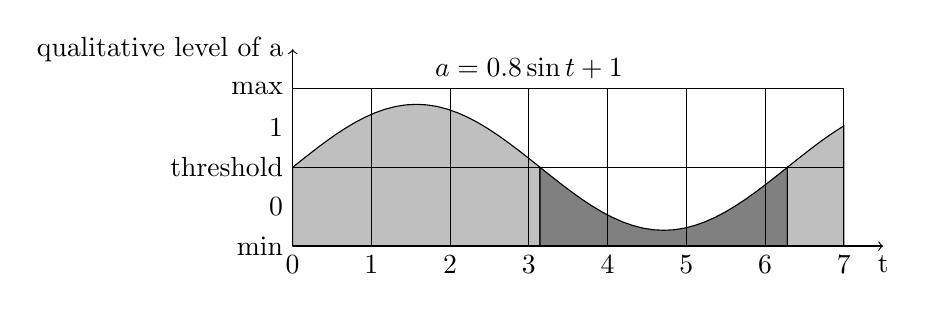
\begin{tikzpicture}
\draw[->] (0,0) -- (0,2.5);
\draw[->] (0,0) -- (7.5,0);
\draw(0,2)node[left]{max};
\draw(0,0)node[left]{min};
\draw(0,1)node[left]{threshold};
\foreach \y in {0,1} \draw(0,\y+0.5)node[left]{\y};
\foreach \x in {0,1,...,7} \draw(\x,0)node[below]{\x};
\filldraw[draw=black,fill=black!25!white]
	plot[domain=0:pi] (\x, {0.8*sin(\x r)+1})--(pi,0)--(0,0)--(0,1); 
\filldraw[draw=black,fill=gray]
	plot[domain=pi:2*pi] (\x, {0.8*sin(\x r)+1})--(2*pi,0)--(pi,0)--(pi,1); 
\filldraw[draw=black,fill=black!25!white]
	plot[domain=2*pi:7] (\x, {0.8*sin(\x r)+1})--(7,0)--(2*pi,0)--(2*pi,1); 
\draw[step=1] (0,0) grid (7,2);
\draw (7.5,0) node[below]{t};
\draw (0,2.5) node[left]{qualitative level of a};
\draw(3,2)node[above]{$a=0.8\sin t+1$};
\end{tikzpicture}
\caption[Variable reconstruction]{Example of variable reconstruction}\label{varRec}
\end{figure}


For the system with 2 Boolean variables $a,b$, the PCCC matrix is created according to Definition \ref{def:corrMatrix}:

%Global state after discretization: $L=\{a_0,a_1\}\times \{b_0,b_1\}\ $

$$\mathcal{R}=\left[
\begin{array}{*{20}c}
r_{a'a} & r_{a'b}\\
r_{b'a} & r_{b'b} \\
\end{array}
\right]\ =\left[
\begin{array}{*{20}c}
{\rm N/A} & r_{a'b}\\
r_{b'a} & {\rm N/A} \\
\end{array}
\right]\ 
$$

After variable reconstruction, the variables are split into four, $a_0,a_1,b_0,b_1$.
The corresponding PCCC matrix $\mathcal{R}'$ is:

$$\mathcal{R}'=\left[
\begin{array}{*{20}c}
r_{a'_0a_0} & r_{a'_0a_1}& r_{a'_0b_0}&r_{a'_0b_1}\\
r_{a'_1a_0} & r_{a'_1a_1}& r_{a'_1b_0}&r_{a'_1b_1}\\
r_{b'_0a_0} & r_{b'_0a_1}& r_{b'_0b_0}&r_{b'_0b_1}\\
r_{b'_1a_0} & r_{b'_1a_1}& r_{b'_1b_0}&r_{b'_1b_1}\\
\end{array}
\right]\ =\left[\begin{array}{*{20}c}
{\rm N/A} & {\rm N/A}& r_{a'_0b_0}&r_{a'_0b_1}\\
{\rm N/A} & {\rm N/A}& r_{a'_1b_0}&r_{a'_1b_1}\\
r_{b'_0a_0} & r_{b'_0a_1}& {\rm N/A}&{\rm N/A}\\
r_{b'_1a_0} & r_{b'_1a_1}& {\rm N/A}&{\rm N/A}\\
\end{array}\right]$$

Here, even though the size of matrix has doubled (it can also be $l$ times large, depending on the number of discrete levels), as the domains of $a_0,a_1,b_0,b_1$ are not continuous and the variables with same origins (like $a_0$ and $a_1$) have no common domain, hence $r_{a_0a_1}$, $r_{a_1a_0}$, $r_{b_0b_1}$, $r_{b_1b_0}$ are meaningless. 
Also, even some variables of from different origins may have no common domain, that will lead to $r_{a_ib_j}=0$, making resulted matrix more sparse, which gives possibilities of optimization.

\subsection{Toy Example}

In order to better illustrate the whole process of generating candidate regulations, a toy example of $4$ variables $a$, $b$, $c$ and $d$ is given below.
To prepare the inputs for the model inference in Section \ref{sec:modelInference} on page \pageref{sec:modelInference}, we want to output candidate regulations.

Input: time series data in Table \ref{TyTable1}, equi-temporal measurement of 8 time units.

Output: candidate regulations for completion by over/under-approximation.

\begin{table}[ht]
\centering
\begin{tabular}{l|*{9}{l}}
$t$&0&1&2&3&4&5&6&7&8\\
\hline
$a$&2.01&2.51&1.97&1.17&0.94&0.70&0.31&0.06&0.06\\
$b$&0.74&0.87&0.78&0.33&0.51&0.82&0.86&1.81&1.08\\
$c$&0.43&0.18&0.42&0.23&0.17&0.23&0.32&0.53&0.80\\
$d$&1.62&1.22&1.07&0.57&0.27&0.28&0.24&0.27&0.31
\end{tabular} 
\caption{Original time-series data generated by Gene Net Weaver \cite{schaffter2011genenetweaver}}\label{TyTable1}
\end{table}

Change rates are obtained in Table \ref{TyTable2} by Equation \ref{eq:changeRate}.

\begin{table}[ht]
\centering
\begin{tabular}{c|c*{7}{S}}
$t$&0&1&2&3&4&5&6&7\\
\hline
$a$&0.5&-0.54&-0.8&-0.23&-0.24&-0.39&-0.25&0.0\\
$b$&0.13&-0.09&-0.45&0.18&0.31&0.04&0.95&-0.73\\
$c$&-0.25&0.24&-0.19&-0.06&0.06&0.09&0.21&0.27\\
$d$&-0.4&-0.15&-0.5&-0.3&0.01&-0.04&0.03&0.04
\end{tabular} 
\caption[Change rates]{Change rates derived from original data by $x'[t]=x[t+1]-x[t]$}\label{TyTable2}
\end{table}

After data regrouping, we obtain 4 matrices with change rate of each variable respectively, four correlation matrices are then computed: 

$$\kbordermatrix{\mbox{}&a'&b&c&d\\
a'&1.0&0.091&-0.296&-0.090   \\
b&0.091&1.0&-0.738&0.423   \\
c&-0.296&-0.738&1.0&-0.383   \\
d&-0.090&0.423&-0.383&1.0
}
\kbordermatrix{\mbox{}&a&b'&c&d\\
a&1.0&0.653&0.896&-0.976   \\
b'&0.653&1.0&0.747&-0.615   \\
c&0.896&0.747&1.0&-0.883   \\
d&-0.976&-0.615&-0.883&1.0 
}$$
$$\kbordermatrix{\mbox{}&a&b&c'&d\\
a&1.0&0.717&-0.561&-0.929   \\
b&0.717&1.0&-0.709&-0.714   \\
c'&-0.561&-0.709&1.0&0.704   \\
d&-0.929&-0.714&0.704&1.0   
}
\kbordermatrix{\mbox{}&a&b&c&d'\\
a&1.0&-0.678&0.780&0.884   \\
b&-0.678&1.0&-0.929&-0.867   \\
c&0.780&-0.929&1.0&0.907   \\
d'&0.884&-0.867&0.907&1.0   
}$$

 $r'$ is formed by taking the $i$-th line from the $i$-th matrix, which suggests the relevance between change rate of one variables and the others.
$$r'=\kbordermatrix{\mbox{}&a&b&c&d\\
a&1.0&0.091&-0.296&-0.090\\
b&0.653&1.0&0.747&-0.615\\
c&-0.561&-0.709&1.0&0.704\\
d&0.884&-0.867&0.907&1.0
}$$
We can set an arbitrary threshold e.g. $0.6$, all the coefficients with their absolute value greater than $0.6$ are listed below:
$$(b,a,0.653),\ (b,c,0.747),\ (b,d,-0.615),\ (c,b,-0.709)$$
$$(c,d,0.704),\ (d,a,0.884),\ (d,b,-0.867),\ (d,c,0.907)$$
For example $(d,b,1,-0.867)$ tells that $d\xrightarrow{-}b$ is probably a good candidate regulation as its absolute value of correlation coefficient is close enough to 1. Like this, a BRN model is formed, see Figure \ref{ResultBRN}. According to the configuration of ABAN (whether absence of regulation is regarded as counter regulation), an ABAN is then deduced.

\begin{figure}[ht]
\centering
\begin{tikzpicture}[grn]
\node[inner sep=0] (a) at (0,0) {a};
\node[inner sep=0] (b) at (2,0) {b};
\node[inner sep=0] (c) at (2,-2) {c};
\node[inner sep=0] (d) at (0,-2) {d};
%\path
%  node[elabel, below=-1em of a] {$0..2$}
%  node[elabel, below=-1em of b] {$0..1$}
%  node[elabel, below=-1em of c] {$0..1$};
\path[->]
  (b) edge node[elabel, above=-3pt] {$+1$} (a)
  (b) edge node[elabel, left=-5pt] {$+1$} (c)
  (b) edge[bend right] node[elabel, above=-3pt] {$-1$} (d)
  (c) edge[bend right] node[elabel, right=-3pt] {$-1$} (b)
  (c) edge node[elabel, above=-5pt] {$+1$} (d)
  (d) edge node[elabel, left=-3pt] {$+1$} (a)
  (d) edge node[elabel, below=-3pt] {$-1$} (b)
  (d) edge[bend right] node[elabel, below=-3pt] {$+1$} (c);
\end{tikzpicture}
\caption{Resulted candidate regulations of the toy example}\label{ResultBRN}
\end{figure}

In fact, the choice of threshold of correlation coefficients has little influence if it is above $0.5$: we can even lower the threshold if resulting regulations do not satisfy desired properties.
Because when coefficient $r =0.5$, then the $95\%$ prediction interval of $y|x$ will be about $13\%$ smaller than the $95\%$ prediction interval of $y$, i.e. $y$ behaves more relevantly than individually \cite{hull1927correlation}.

It is worth noticing that this method does not take into account the interactions between regulations, i.e. we do not distinguish between the conjunctions and disjunctions.
For candidate regulations $(a,c,+)$ and $(b,c,+)$, the following set of transitions are both consistent \{\ac{a_1,b_1}{c_0}{c_1}\} and \{\ac{a_1}{c_0}{c_1}, \ac{b_1}{c_0}{c_1}\}.
In CRAC, we do not consider conjunctions for candidate regulations.

Last but not least, the high-correlated variable pairs are not necessarily the reality but can also be a coincidence, i.e. the inferred candidate regulations/transitions can probably reproduce the system dynamics but cannot guarantee the identity.
In fact, there is no method that can guarantee it reveals the reality, as what model inference does is to infer \textit{via} the correlations instead of causality.
Causality, or the reason behind the observation is very hard to retrieve.

\section{Model Revision \textit{via} Reachability and Interpretation Transitions (M2RIT)}
When modeling a real system, instead of causality, one usually require to assess the \textit{consistency} between a given modeling network and the concrete system by checking whether the observed configurations are indeed reachable in the Boolean network.
Whenever it is not the case, it typically means that the designed Boolean functions do not model the given system correctly and thus should be revised before further model analysis.

Inoue \cite{inoue2011logic} has shown that Boolean networks can be represented by logic programs.
In this paper, we provide an approach to revise a logic program to fit temporal properties regarding reachability of partial states.
%
Such logic program can be learned from observations of state transition using LFIT algorithm in \cite{ribeiro2015learning}, but the approach restricts the model to only synchronous update scheme.
One of the benefits of synchronous modeling is computational tractability, while classical state space exploration algorithms fail on asynchronous ones.

Yet the synchronous modeling relies on quite heavy assumptions:
all genes can make a transition simultaneously and need an equivalent amount of time to change their expression level.
Even if this is not realistic from a biological point of view, it is usually sufficient as the exact kinetics and order of transformations are generally unknown.
However, asynchronous semantics helps one to capture more realistic behaviors \cite{bernot2009}.
At a given time point, at most one single gene can change its expression level.
Non-deterministic behaviors are often observed in biological systems, e.g. cell differentiation.
From a given state, several possible behaviors can be expected as future states.
Asynchronous update scheme results in a potential combinatorial explosion to the number of states.

Considering the ignorance of conjunctions by CRAC, we use a more precise learning technique (LFIT) to obtain the model to be revised in M2RIT.
The trade-off is that M2RIT cannot deal with noisy data sets and there are more constraints in the revision phase because we have to keep the consistency of the resulted network with the original time-series data.

Here we follow the same methodology as shown in Figure \ref{fig:bigPicture} on page \pageref{fig:bigPicture}.
First we obtain the model to be revised via learning method LFIT, then we modify the learned transitions according to the SLCG but in a way that maintaining the revised model can always reproduce the original time-series data.

\subsection{Learning From Interpretation Transitions (LFIT)}\label{sec:lfit}
LFIT framework so far can only capture finite dynamical properties, i.e. relation at $T$-$1$ or $T$-$k$ and the system has to be synchronous deterministic.
In asynchronous systems, non-determinism can lead to loops for several times before taking a path to a certain state.
In this thesis, we adapt the algorithms of \cite{ribeiro2015learning,DMTRICLP15} to capture asynchronous dynamics and extend upon this method to propose an approach allowing to fit a logic program to reachability properties.
By modifying rules of the program using logic generalization/specialization operations, we iteratively revise the program to fit a set of reachability/unreachability constraints while keeping the observation and the learned rules consistent.

\subsection{Formalization}
    
	Boolean asynchronous systems can be non-deterministic, thus from the same state a variable can take both value $0$ or $1$.
	To encode this dynamics, one requires to have explicit rules for each value of a variable and the modeling of \cite{ribeiro2015learning} is not suitable.
	Mart{\'\i}nez \textit{et al.} \cite{DMTRICLP15} have proposed a modeling of multi-valued synchronous systems as annotated logic program.
    This modeling can be applied to represent Boolean asynchronous systems and is recalled in the following section.
    %
	In order to represent multi-valued variables, all atoms of a logic program are now restricted to the form $var^{val}$.
	The intuition behind this form is that $var$ represents some variable of the system and $val$ represents the value of this variable.
	In annotated logics, the atom $var$ is said to be annotated by the constant $val$.
	Let us consider a {\it multi-valued logic program\/} as a set of {\it rules\/} of the form  
	\begin{equation}\label{multi_value}
		var^{val} \leftarrow var_1^{val_1} \wedge \cdots \wedge var_n^{val_n}
	\end{equation}
	where $var^{val}$ and $var_i^{val_i}$ are atoms $(n \geq 1)$.
	For any rule $R$ of the form~(\ref{multi_value}), left part of $\leftarrow$ is called the {\it head\/} of $R$ and is denoted as $h(R)$,
	and the conjunction to the right of $\leftarrow$ is called the {\it body\/} of $R$.  
	We represent the set of literals in the body of $R$ of the form~(\ref{multi_value}) as $b(R)=\{var_1^{val_1},\ldots,var_n^{val_n}\}$. 
	A rule $R$ of the form (\ref{multi_value}) is interpreted as follows:
	the variable $var$ takes the value $val$ in the next state if all variables $var_i$ have the value $val_i$ in the current state.
	A state of a multi-valued program provides the value of each variable of the system and a transitions is a pair of states.
	The value of a variable in a state is called a local state.
	The set of all local states is denoted $\mathbf{LS}$.
	The subset of a state is called a partial state.
	A rule $R$ matches a state $s$ when $b(R) \subseteq s$.
	A rule $R$ subsumes a rule $R'$ when $h(R)=h(R'), b(R) \subseteq b(R')$.
%
A Boolean Asynchronous system can be represented by a multi-valued logic program.
This section provides the necessary additional formalization to interpret asynchronous dynamics by such program and to learn from state transitions.

\subsection{Modeling and Learning of Asynchronous Dynamics}\label{sec:alfit}

Due to the non-deterministic nature of asynchronous systems and its restriction to atmost one variable change per transition,
the notions of consistency, realization and successor have to be adapted as follows.

\begin{definition}[Consistency]
	Let $R$ be a rule and $E$ be a set of state transition $(I,J)$.
	$R$ is {\it consistent} with $E$ iff
	$b(R)\subseteq I$ implies $\exists (I,J) \in E, h(R) \in J$.
	A logic program $P$ is {\it consistent} with $E$ if all rules of $P$ are {\it consistent} with $E$.
\end{definition}

\begin{definition}[Program realization]
	Let $P$ be a logic program and $E$ be a set of state transitions.
	$P$ realizes $E$ if $\forall (I,J) \in E, \exists R, b(R) \subseteq I, (I \setminus J) = \{h(R)\}$.
\end{definition}

\begin{definition}[Asynchronous successors]
	Let $I$ be the current state of an asynchronous system represented by a set of multi-valued rules $S$.
	Let $T_P(I,S) = \{h(R) | R \in S, b(R) \subseteq I\}$.
	The successors of $I$ according to $S$ is
	$$T_P^{as}(I,S) = \{I \setminus \{v^{val'}\} \cup \{v^{val}\} | v^{val'} \in I, v^{val} \in T_P(I,S)\} \cup \{I \mid T_P(I,S) = \emptyset\}$$ % Self loop only for non-point atractor
\end{definition}

We now adapt the {\bf LFIT} algorithm of \cite{ribeiro2015learning} to the learning of asynchronous systems.
In synchronous case, the rules $R$ learned by {\bf LFIT} represent a necessity: $h(R)$ \textit{will} be in the next state if $R$ match the current state.
In asynchronous case, the rules represent a possibility: $h(R)$ \textit{can} be in next state if $R$ match the current state.
It allows the modeling of non-determinism: two rules $R, R'$ can have the same head variables but different values and match the same state which occurs in these case:
$h(R)=var^{val}, h(R')=var^{val'}, val \neq val'$ and $var^{val''} \in b(R), var^{val'''}\in b(R') \implies val'' = val'''$.

Like in previous versions, {\bf LFIT} takes a set of state transitions $E$ as input and outputs a logic program $P$ that realizes $E$.
In \cite{DMTRICLP15} multi-valued least specialization was used to learn multi-valued {\bf synchronous} systems dynamics.
Starting from the most general rules, least specialization allows to learn the minimal rules of such system iteratively from its state transition $(I,J) \in E$.
For every possible $var^{val}$, $var^{val} \not \in J$ the most specific rule that is not consistent, with the transition, i.e. an anti-rule, was generated: $MSR := var^{val} \leftarrow I$.
Here, for the {\bf asynchronous} case, this anti-rule is generated and the revision occurs only if $\nexists (I,J') \in E, var^{val'} \in J'$,
i.e. it is impossible to have a transition to $var^{val}$ from $I$.
Each rule of the currently learned program $P$ that subsumes such an anti-rule are specialized using least specialization.
The resulting program $P'$ is consistent and realizes all previously treated transition plus $(I,J)$.
By doing so iteratively for each transition, the algorithm outputs a program $P$ which models the dynamics of the system observed in the transitions $E$.

\vspace{0.5em}
\noindent
\textbf{Asynchronous LFIT}
\vspace{-0.4em}
\begin{itemize}
	\item INPUT: $\mathcal{B}$ a set of annotated atoms and $E$ a set of transitions
	\item Initialize $P := \{var^{val} \leftarrow \emptyset \mid var^{val} \in \mathcal{B}\}$
	\item For each $(I,J) \in E$
	\begin{itemize}
		\item For each $var^{val} \in \mathcal{B}$
		\begin{itemize}
			\item If $\nexists (I,J') \in E, var^{val} \in J'$
			\item $MSR := var^{val} \leftarrow I$
			\item Extract each rule $R$ of $P$ that subsumes $MSR$: $MR := \{R \in P \mid h(R) = var^{val}, b(R) \subseteq I\}, P := P \setminus MR$
			\item For each $R \in MR$
			\begin{itemize}
				\item Compute its least specialization $P'=ls(R,MSR,\mathcal{B})$.
				\item Remove all the rules in $P'$ subsumed by a rule in $P$.
				\item Remove all the rules in $P$ subsumed by a rule in $P'$.
				\item Add all remaining rules in $P'$ to $P$.
			\end{itemize}
		\end{itemize}
	\end{itemize}
	\item OUTPUT: $P$
\end{itemize}

\begin{definition}[Consistent program]
Let $P$ be a logic program, $Re$ (resp. $Un$) be a set of reachability (resp. unreachability) properties.
$P$ is said to be {\em consistent} with $Re$ (resp. $Un$) iff
$\forall (\alpha,\omega) \in Re, \exists$ a trajectory $t$ in $P$ s.t. $\alpha.t=\omega$ and 
$\forall (\alpha,\omega) \in Un, \nexists$ a trajectory $t$ in $P$ s.t. $\alpha.t=\omega$.
\end{definition}

Specializing a rule is to add elements in the body of a rule,
thus to make the condition of a rule more difficult to be satisfied (in a more specialized situation) as the condition of firing becomes more strict.

\begin{definition}[Least specialization of a rule]
	Let $R$ be a rule, a least specialization of $R$ is a rule $R' \in ls(R) := \{h(R) \leftarrow b(R) \cup \{var^{val}\}, \nexists var^{val'} \in b(R)\}$.
	If $R$ contains already all the variables in its body, the only way to specialize $R$ is to remove $R$.
\end{definition}

    Similarly, generalization of a rule is to remove certain elements in the body of a rule, thus to make the condition of a rule easier to be satisfied.

\begin{definition}[Least generalization of a rule]
	Let $R$ be a rule, a least generalization of $R$ is a rule $R' \in lg(R) := \{h(R) \leftarrow b(R) \setminus \{x\},  x \in b(R)\}$.
\end{definition}

\begin{definition}[Revisable]\label{def:revisable}
	A logic program $P$ is said revisable w.r.t. a reachability (resp. unreachability) property if:
	$\exists P' \in \{(P \setminus R_P) \cup \{R' \mid R \in R_P, R' \in ls(R) \cup lg(R)\} \} \mid R_P \subseteq P\}$.
	$P$ is revisable w.r.t. to a set of property $S$:
	if their exists an ordering $S'$ of the elements of $S$ such that each $i$th revision, $0 \leq i \leq |S'|$, ($P$ being the $0$th revision) is revisable w.r.t. the $i+1$th property.
\end{definition} 

From definition \ref{def:revisable}, it follows that the revision of logic program $P$ w.r.t. a set of reachability/unreachability properties $S$ can be found (or proved to be non-existent) by brute force enumeration of all possible ordering of $S$ and trying all possible iterative revisions of $P$.
In the next section we propose an algorithm exploiting the SLCG structure to restrict the search to valid ordering of the properties.
\subsection{Revision}
\label{sec:algorithm}

    In this section, we are going to present our algorithm \textbf{M2RIT} (\textbf{M}odel \textbf{R}evision \textit{via} \textbf{R}eachability and \textbf{I}nterpretation \textbf{T}ransitions) exploiting the previous formalization to fit a logic program to reachability properties.
    Given a set of transition $E$ of an asynchronous system $S$, a logic program $P$ is learned via the adaptation of \textbf{asynchronous LFIT} of section \ref{sec:alfit}.
    When $E$ is partial, the learned program $P$ does not have the exact dynamics of $S$.
    Given a set of reachability properties $Re$ and a set of unreachability properties $Un$ of $S$, we propose an algorithm to revise $P$ so that the dynamics of $P$ satisfy $S$.
    As discussed previously, this can be done by complete brute force but here we propose a first attempt to reduce the search space.
	% TODO: detail why ordering is correct, notion of precedence and so on
    Furthermore, our aim is to find what could be considered a metric of minimal revision of $P$:
    a revision $P'$ s.t. $\nexists P'', (P''\setminus P \cap P'')\subseteq (P' \setminus P \cap P')$
   
    Specialization/generalization operations aim to revise the rule nearest to the target state in the SLCG. If it is not possible, they try to revise the successor, if there is no possible solution, return $\varnothing$ to show the input logic program is not revisable. Specialization operation is limited by the observation. If $P$ after specialization can not explain all the transitions, the specialization is not admissible. %When specializing one rule, we check if all appeared transitions are explained, if not, check if there are other rules can explain it, otherwise we can not specialize it.
    Generalization is similar but without the constraint of the observation, as the observation is partial, $P$ may describe some state transitions never observed.
   
    Specialization:
    \begin{itemize}
        \item \textbf{Input}: a logic program $P$, an unsatisfied element $(\alpha,\omega)$, a reachable set $Re$, an unreachable set $Un$%, a maximum addable variables $k$
        \item \textbf{Output}: modified logic program $P$ or $\varnothing$ if not revisable
    \end{itemize}
    \begin{enumerate}
        \item $Rev\gets\{\omega\}$
        \item \textbf{For} each $R$ s.t. $h(R)=Rev$, for each $R'\in\{R''|R''\in ls(R)\land \nexists (I,J)\in E, \text{ s.t. } \nexists R'''\in P\cup \{R''\}\setminus \{R\}, h(R''')\in J, b(R''')\in I\}$
        \begin{itemize}
            \item \textbf{If} $P' \gets P \setminus \{R\} \cup \{R'\}$, $unreachable(P',\alpha,\omega$) and $P'$ satisfies all previous properties, \textbf{return} $P'$
        \end{itemize}
        \item $Rev\gets b(R)$ with $h(R)=Rev$ and back to step 2
        \item There is no revision for $(\alpha,\omega)$, \textbf{return} $\varnothing$
    \end{enumerate}
    Generalization:
    \begin{itemize}
        \item \textbf{Input}: a logic program $P$, an unsatisfied element $(\alpha,\omega)$, a reachable set $Re$, an unreachable set $Un$
        \item \textbf{Output}: modified logic program $P$ or $\varnothing$ if not revisable
    \end{itemize}
    \begin{enumerate}
        \item $Rev\gets\{\omega\}$
        \item \textbf{For} each $R$ s.t. $h(R)=Rev$, for each $R'\in lg(R)$
        \begin{itemize}
            \item \textbf{If} $P' \gets P \setminus \{R\} \cup \{R'\}$, $reachable(P',\alpha,\omega$) and $P'$ satisfies all previous properties, \textbf{return} $P'$
        \end{itemize}
        \item $Rev\gets b(R)$ with $h(R)=Rev$ and back to step 2
        \item There is no revision for $(\alpha,\omega)$, \textbf{return} $\varnothing$
    \end{enumerate}
    Complete revision:
    \begin{itemize}
        \item \textbf{Input}: a logic program $P$, a reachable set $Re$ and an unreachable set $Un$
        \item \textbf{Output}: revised logic program $P$ or $\varnothing$ if not revisable
    \end{itemize}
    \begin{enumerate}
        \item Construct the cycle-free SLCGs for the elements in $Re$ and $Un$ and compute unsatisfied sets $Re'\subseteq Re$ and $Un'\subseteq Un$ which are to be revised
        \item \textbf{If} $Re'=\varnothing$ and $Un'=\varnothing$, \textbf{return} $P$
        \item Let $L=\{l_i,\ldots\}$ with $i\in Re' \cup Un'$, $l_i=\{j,\ldots\}$, with $j=(\alpha,\omega)$, $\omega \in SLCG(i)$ and $ j\in Re\cup Un$ \label{step:dependency}
        \item Pick one of $l_i\in L$ of the smallest cardinality: $\nexists l_i'$, $|l_i'| < |l_i|$ \label{step:cardinality}
        \item \textbf{If} $l_i\cap (Re'\cup Un')\neq\varnothing$, \label{step:check}
        \begin{enumerate}
            \item Reconstruct the SLCG for $i$
            \item \textbf{If} $l_i$ becomes consistent because of former revision, $L\gets L\setminus \{l_i\}$ and back to step 4
        \end{enumerate}
        \item \textbf{If} $i\in Un'$, specialize $P$ to make $i$ unreachable, \textbf{if} not revisable, \textbf{return} $\varnothing$ \label{step:specialize}
        \item Otherwise generalize $P$ to make $i$ reachable, \textbf{if} it is not revisable, \textbf{return} $\varnothing$ \label{step:generalize}
        
        \item $L\gets L\setminus\{l_i\}$ \label{step:update}
        \item \textbf{If} $L\neq\varnothing$ , back to step 1 \label{step:recheck}
        \item \textbf{Return} $P$
    \end{enumerate} 
%        \noindent
%    \begin{minipage}{\linewidth}
%    Specialization:
%    \begin{itemize}
%        \item \textbf{Input}: a logic program $P$, an unsatisfied element $(\alpha,\omega)$, a reachable set $Re$, an unreachable set $Un$%, a maximum addable variables $k$
%        \item \textbf{Output}: modified logic program $P$ or $\varnothing$ if not revisable
%    \end{itemize}
%    \begin{enumerate}
%        \item $Rev\gets\{\omega\}$
%        \item \textbf{For} each $R$ s.t. $h(R)=Rev$, for each $R'\in\{R''|R''\in ls(R)\land \nexists (I,J)\in E, \text{ s.t. } \nexists R'''\in P\cup \{R''\}\setminus \{R\}, h(R''')\in J, b(R''')\in I\}$
%        \begin{itemize}
%            \item \textbf{If} $P' \gets P \setminus \{R\} \cup \{R'\}$, $unreachable(P',\alpha,\omega$) and $P'$ satisfies all previous properties, \textbf{return} $P'$
%        \end{itemize}
%        \item $Rev\gets b(R)$ with $h(R)=Rev$ and back to step 2
%        \item There is no revision for $(\alpha,\omega)$, \textbf{return} $\varnothing$
%    \end{enumerate}
%    \end{minipage}
%    \noindent
%    \begin{minipage}{\linewidth}
%    Generalization:
%    \begin{itemize}
%        \item \textbf{Input}: a logic program $P$, an unsatisfied element $(\alpha,\omega)$, a reachable set $Re$, an unreachable set $Un$
%        \item \textbf{Output}: modified logic program $P$ or $\varnothing$ if not revisable
%    \end{itemize}
%    \begin{enumerate}
%        \item $Rev\gets\{\omega\}$
%        \item \textbf{For} each $R$ s.t. $h(R)=Rev$, for each $R'\in lg(R)$
%        \begin{itemize}
%            \item \textbf{If} $P' \gets P \setminus \{R\} \cup \{R'\}$, $reachable(P',\alpha,\omega$) and $P'$ satisfies all previous properties, \textbf{return} $P'$
%        \end{itemize}
%        \item $Rev\gets b(R)$ with $h(R)=Rev$ and back to step 2
%        \item There is no revision for $(\alpha,\omega)$, \textbf{return} $\varnothing$
%    \end{enumerate}
%    \end{minipage}
%    \noindent
%    \begin{minipage}{\linewidth}
%    Complete revision:
%    \begin{itemize}
%        \item \textbf{Input}: a logic program $P$, a reachable set $Re$ and an unreachable set $Un$
%        \item \textbf{Output}: revised logic program $P$ or $\varnothing$ if not revisable
%    \end{itemize}
%    \begin{enumerate}
%        \item Construct the cycle-free SLCGs for the elements in $Re$ and $Un$ and compute unsatisfied sets $Re'\subseteq Re$ and $Un'\subseteq Un$ which are to be revised
%        \item \textbf{If} $Re'=\varnothing$ and $Un'=\varnothing$, \textbf{return} $P$
%        \item Let $L=\{l_i,\ldots\}$ with $i\in Re' \cup Un'$, $l_i=\{j,\ldots\}$, with $j=(\alpha,\omega)$, $\omega \in SLCG(i)$ and $ j\in Re\cup Un$ \label{step:dependency}
%        \item Pick one of $l_i\in L$ of the smallest cardinality: $\nexists l_i'$, $|l_i'| < |l_i|$ \label{step:cardinality}
%        \item \textbf{If} $l_i\cap (Re'\cup Un')\neq\varnothing$, \label{step:check}
%        \begin{enumerate}
%            \item Reconstruct the SLCG for $i$
%            \item \textbf{If} $l_i$ becomes consistent because of former revision, $L\gets L\setminus \{l_i\}$ and back to step 4
%        \end{enumerate}
%        \item \textbf{If} $i\in Un'$, specialize $P$ to make $i$ unreachable, \textbf{if} not revisable, \textbf{return} $\varnothing$ \label{step:specialize}
%        \item Otherwise generalize $P$ to make $i$ reachable, \textbf{if} it is not revisable, \textbf{return} $\varnothing$ \label{step:generalize}
%        
%        \item $L\gets L\setminus\{l_i\}$ \label{step:update}
%        \item \textbf{If} $L\neq\varnothing$ , back to step 1 \label{step:recheck}
%        \item \textbf{Return} $P$
%    \end{enumerate} 
%    \end{minipage}
      
    The main algorithm starts with constructing the SLCGs to verify $Re$ and $Un$ in order to ensure the reachability/unreachability properties to be satisfied.
    Then, for the unsatisfied properties, the program $P$ has to be revised.
    SLCG can share the elements s.t. revising one can modify the others.
    By starting with the SLCGs with least dependencies with others, i.e. the ones with the smallest cardinality of $l_i$, it increases the chance of partially satisfying other unsatisfied properties (step \ref{step:dependency} and \ref{step:cardinality}). 
    Then all possible revision of $P$ are generated using least specialization or generalization according to $l_i\in Re$ or $l_i \in Un$ (step \ref{step:specialize} and \ref{step:generalize}). 
    Each revision of $P$ is checked against $Re$ and $Un$ to verify that all properties satisfied by $P$ are still satisfied. 
    If new ones are satisfied, $L$ is updated accordingly (step \ref{step:check}).
    We update $P$ until there is no unsatisfied properties (step \ref{step:update} and \ref{step:recheck}).
    %As the SLCGs are free of cycles, the algorithm always terminates.
    %we revise first the elements whose SLCG contain least other elements in order to modify less $P$.
    Finally, if a revision of $P$ consistent with all given properties is found the algorithm terminates and outputs it.
    
\subsection{Toy Example}    
\textbf{Some explanation}
    \begin{figure}[ht]
        \centering
        \begin{tikzpicture}[aS]  
  	\node[Aproc] (a_1) {$a_1$};
  	\node[Asol,right of = a_1] (a_1s) {};
  	\node[Asol,below right of = a_1] (a_1s2) {};
  	\path (a_1) edge (a_1s);
  	\path[thick,dashed,color=blue] (a_1) edge (a_1s2);
  	%\path (a_1) edge (a_1s2);
  	\node[Aproc,right of = a_1s2] (d_1) {$d_1$};
  	\node[Aproc,below right of = a_1s2] (c_0) {$c_0$};
  	\node[Asol,right of = c_0] (c_0s) {};
  	%\path<3>[thick,dashed,color=green] (a_1s2) edge (d_1);
  	\draw[->,thick,dashed,color=red] (a_1s2) to node[color=black] {\LARGE $\times$} (d_1);
  	%\path (a_1s2) edge (d_1);
  	\path (a_1s2) edge (c_0);
  	\path (c_0) edge (c_0s);
  	\edl{c_0};
  	\node[Aproc,right of = a_1s] (b_1) {$b_1$};
  	\path (a_1s) edge (b_1);
  	\node[Asol, right of = b_1] (b_1s) {};
  	\path[thick,dashed,color=blue] (b_1) edge (b_1s);
  	%\path (b_1) edge (b_1s);
  	\link{b_1}{c_0};
 	\edl{c_0};
 	\node[Aproc,below right of = b_1s] (a_1) {$a_1$};
 	%\node[Asol,right of = c_1] (c_1s) {};
 	\path[thick,dashed,color=green] (b_1s) edge (a_1);
 	%\path (b_1s) edge (a_1);
 	%\path (c_1) edge (c_1s);
 	%\node[Aproc,right of = c_1s] (a_1) {$a_1$};
 	%\path (c_1s) edge (a_1);
	%\link{a_1}{c_1};
	%\link{c_1}{a_1};
 	%\edl{a_1};
\end{tikzpicture}
        \caption{Toy example of M2RIT (Explanation of legends)}
        \label{fig:toyExampleM2RIT}
    \end{figure}
\section{R\'esum\'e}
In this chapter we presented three approaches to infer/revise models based on different \textit{a priori} knowledge.
The first approach allows one to construct a good model among a large number of candidate transitions.
The drawback of the first approach is to obtain the candidates.
To cover this disadvantage, the statistic approach \textit{via} correlation coefficients provides us with candidate regulations to be verified by the first approach.
The statistic approach can use all the continuous time-series data to construct a model from nothing but hard to take into account additional constraints.
The first two approaches are combined as \textbf{CRAC} (\textbf{C}ompletion \textit{via} \textbf{R}eachability \textbf{A}nd \textbf{C}orrelations)

Considering the disadvantages of the combination of CRAC, the third approach \textbf{M2RIT} (Model Revision \textit{via} Reachability and Interpretation Transitions) does not need candidate transitions and can adjust the result by reachability constraints.
It revises the logic program learned by LFIT w.r.t. the knowledge on reachability properties.
When talking about reachability, we should fix at first update scheme of the dynamic system.
We use asynchronicity as the update scheme as it implies non-determinism which is meaningful to the modeling of nuanced uncertain parts in biology.
From the point of view of revisability, asynchronicity gives the possibilities of modifying the existing transitions.
If the logic program is revisable, the revision is consistent with both state transitions and reachability information.
Intuitively speaking, a given set of time-series data is usually consistent with less synchronous systems than asynchronous systems, thus it is more likely to revise a asynchronous system to satisfy certain reachabilty constraints.

The drawback of M2RIT is that there is a loss of information due to discretization, while the first two approaches make full use of the continuous data.
Moreover, M2RIT does not guarantee the minimal revision of the logic program.

From the contents of this chapter, we propose several topics as future work
\begin{itemize}
    \item Developing heuristics to improve the performance of the existing algorithms
    \item Considering the metric for minimal revision and designing a related algorithm
    \item Reachability in the meaning of continuous models
    \item Adapting more dynamical properties other than reachability
\end{itemize}